\documentclass{beamer}

\mode<presentation> {%
	\usetheme{Frankfurt}
}

% \usepackage{times}
\usepackage{amsmath,amssymb}
\usepackage[english]{babel}
\usepackage[utf8]{inputenc}
% \usepackage[latin1]{inputenc}

\usepackage{fancybox}
\usefonttheme[onlymath]{serif}
\boldmath

\usepackage{scalefnt}
\usepackage{ragged2e}
\usepackage{graphics}
\usepackage{url}
\usepackage{graphicx}
\usepackage{mathrsfs}
\usepackage{amsfonts}
\usepackage[authoryear,round]{natbib}

\usepackage[group-separator={,}]{siunitx}
\usepackage{caption}
\usepackage{pbox}
\usepackage{tabularx}

\usepackage{color}

\graphicspath{{../../Agranda2016/}{../../Agranda2016/workshop_data_science/}}

\captionsetup[figure]{labelformat=empty}% redefines the caption setup of the figures environment in the beamer class.

\newcommand{\Beta}{B}

\newcommand{\mathA}{\mathcal{A}}
\newcommand{\mathB}{\mathcal{B}}
\newcommand{\mathC}{\mathcal{C}}
\newcommand{\mathG}{\mathcal{G}}
\newcommand{\mathP}{\mathcal{P}}

\newcommand{\TP}{\operatorname{TP}}
\newcommand{\TN}{\operatorname{TN}}
\newcommand{\FP}{\operatorname{FP}}
\newcommand{\TPR}{\operatorname{TPR}}
\newcommand{\FPR}{\operatorname{FPR}}
\newcommand{\AUC}{\operatorname{AUC}}

\newcommand{\closeopen}[2]{\left[ #1, #2 \right)}

\usepackage{array}
\newcolumntype{L}[1]{>{\raggedright\let\newline\\\arraybackslash\hspace{0pt}}m{#1}}
\newcolumntype{C}[1]{>{\centering\let\newline\\\arraybackslash\hspace{0pt}}m{#1}}
\newcolumntype{R}[1]{>{\raggedleft\let\newline\\\arraybackslash\hspace{0pt}}m{#1}}

\beamertemplatenavigationsymbolsempty

%%%%%%%%%%%%%%%%%%%%%%%%%%%%%%%%%%%%%%%%%%%%%%%%%%%%%%%%%%%%%%%%%%%%%%%%%%%%%%%%%%%%%%%%%%%%%%%%%%%%%%%%%%%%
%%%%%%%%%%%%%%%%%%%%%%%%%%%%%%%%%%%%%%%%%%%%%%%%%%%%%%%%%%%%%%%%%%%%%%%%%%%%%%%%%%%%%%%%%%%%%%%%%%%%%%%%%%%%

  \title{A Bayesian Approach to Income Inference \\ in a Communication Network}

\author[Fixman et.\ al]{%
	Martin~Fixman\inst{1}\inst{2}\and
	Ariel~Berenstein\inst{1}\and
	Jorge~Brea\inst{1}\and
	Martin~Minnoni\inst{1}\and
	Matias~Travizano\inst{1}
	Carlos~Sarraute\inst{1}\and
}

\institute{%
	\inst{1}Grandata, Buenos Aires and San Francisco \\
	\inst{2}Universidad de Buenos Aires, Argentina 
}

\bigskip

  \date{IEEE/ACM ASONAM 2016 \\ 21 August 2016}


%\setbeamertemplate{footline}[text line]{\bf \insertshortauthor \hfill \insertshorttitle \hfill \insertframenumber/29}
\setbeamertemplate{footline}[text line]{\hfill \insertframenumber / 30}

\AtBeginSection[]
{%
  \begin{frame}<beamer>{Agenda}
    \tableofcontents[currentsection]
  \end{frame}
}
  
%%%%%%%%%%%%%%%%%%%%%%%%%%%%%%%%%%%%%%%%%%%%%%%%%%%%%%%%%%%%%%%%%%%%%%%%%%%%%%%%%%%%%%%%%%%%%%%%%%%%%%%%%%%%
%%%%%%%%%%%%%%%%%%%%%%%%%%%%%%%%%%%%%%%%%%%%%%%%%%%%%%%%%%%%%%%%%%%%%%%%%%%%%%%%%%%%%%%%%%%%%%%%%%%%%%%%%%%%
%%%%%%%%%%%%%%%%%%%%%%%%%%%%%%%%%%%%%%%%%%%%%%%%%%%%%%%%%%%%%%%%%%%%%%%%%%%%%%%%%%%%%%%%%%%%%%%%%%%%%%%%%%%%
\begin{document}


\begin{frame}
\titlepage
\end{frame}



%%%%%%%%%%%%%%%%%%%%%%%%%%%%%%%%%%%%%%%%%%%%%%%%%%%%%%%%%%%%%%%%%%%%%%%%%%%%%%%%%%%%%%%%%%%%%%%%%%%%%%%%%%%%
\section{Introduction}
%%%%%%%%%%%%%%%%%%%%%%%%%%%%%%%%%%%%%%%%%%%%%%%%%%%%%%%%%%%%%%%%%%%%%%%%%%%%%%%%%%%%%%%%%%%%%%%%%%%%%%%%%%%%

\begin{frame}{Presentation}

\begin{block}{About Grandata}
\begin{itemize}

\item Founded in 2012.

\item Labs and Data Science team:
\begin{itemize}
\item 5 persons, based in Buenos Aires, Argentina~\ldots \\ and now in San Francisco!
\item $\forall$ students and PhDs from FCEyN, UBA \\ $\in$ Computer Sc., Physics, Mathematics
\end{itemize}

\item Researching Human Dynamics
\begin{itemize}
\item Using ``Big Data'' to analyze social networks and human behavior.
\item Integrating banking and cellphone data.
\item We aim to characterize users and predict user actions.
\end{itemize}

\end{itemize}

\end{block}
\end{frame}


\begin{frame}{Human Behavior}

\begin{tabularx}{\textwidth}{c c}
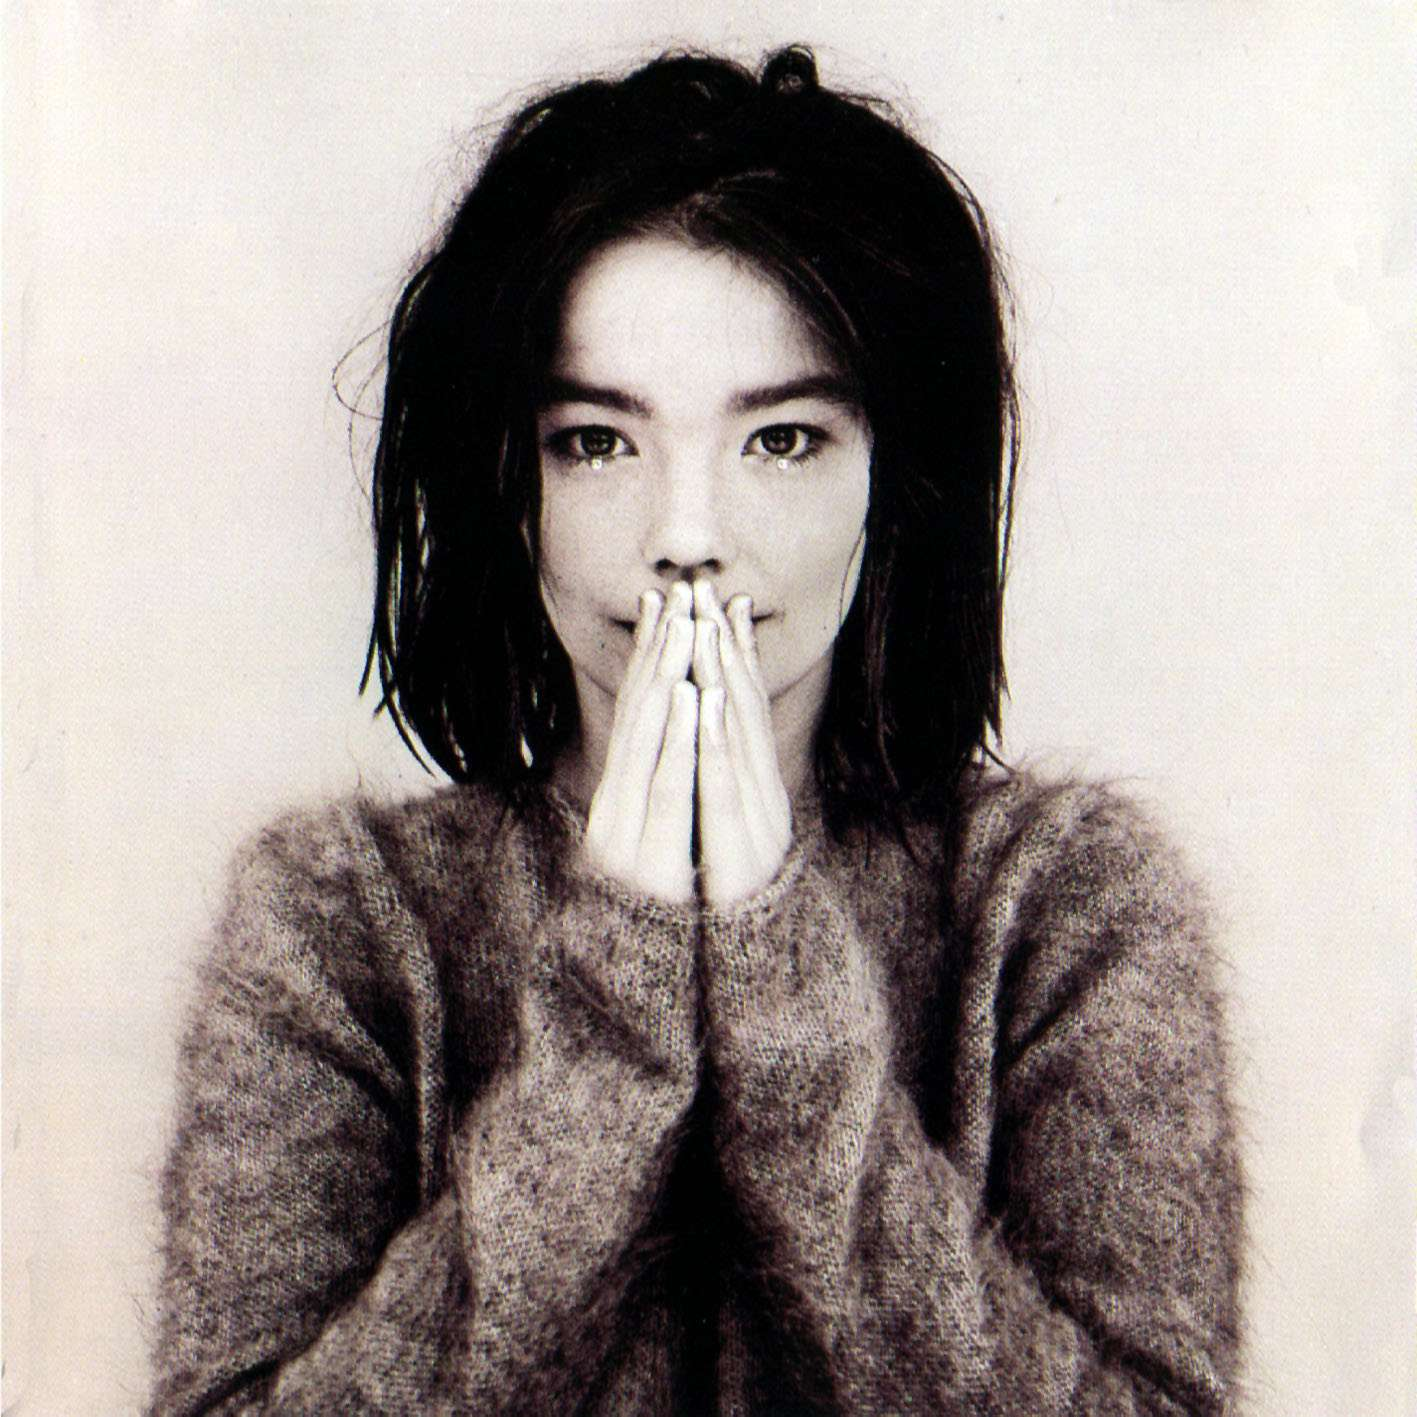
\includegraphics[height=0.4\textheight]{bjork-debut.jpg} &
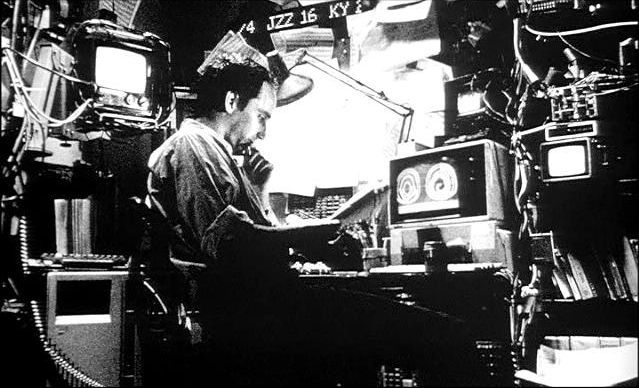
\includegraphics[height=0.4\textheight]{pi.jpg} \\

\pbox[t]{0.4\textwidth}{%
\small
There's definitely, definitely, definitely no logic \\
to human behavior \\
\\
\textit{Björk --- Debut}
} &
\pbox[t]{0.6\textwidth}{%
\small
Restate my assumptions: \\
1. Mathematics is the language of nature. \\
2. Everything around us can be represented and understood through numbers. \\
3. If you graph the numbers of any system, patterns emerge. \\
\\
\textit{Aronofsky --- Pi}
}
\end{tabularx}

\end{frame}

\begin{frame}{The Scientific Connection}
\begin{block}{Scientific Collaborations}
\begin{itemize}
\item Aline Viana (Inria, Paris)
\item Eric Fleury, Marton Karsai (ENS,Lyon)
\item Sandy Pentland and the Human Dynamics team (MIT)
\item Marta Gonzalez and the Human Mobility team (MIT)
\item Alejo Salles and Pablo Groisman (UBA)
\item Mundo Sano Foundation
\end{itemize}
\end{block}

\pause

\begin{block}{Publications}
\begin{itemize}
\item 30 papers published
\item Conferences: NetMob, ASONAM, KDD, \ldots
\item Journals: AI Communications, Elsevier Computer Communications, \ldots
\item 4 papers here at ASONAM
\end{itemize}
\end{block}

\bigskip

\cite{leo2015socioeconomic}
\cite{gonzalez2008understanding,sarraute2015city}
\cite{mcpherson2001birds}
\cite{sarraute2014}

\end{frame}


\begin{frame}{Summary}

\begin{itemize}

\begin{block}{Objective}
Generate inferences of socioeconomic status in the communication graph.
\end{block}
\medskip

\pause

\item Use 2 data sources:
\begin{itemize}
\item Call Detail Records (CDRs) from the operator allow us to construct a social graph.
\item Banking reported income for a subset of clients obtained from a large bank.
\end{itemize} 

\item We construct an \textcolor{blue}{inference algorithm} that allows us to predict the socioeconomic status of users.

\item The first time that both mobile phone and banking information has been integrated in this way to make inferences based on a social telecommunication graph.

\end{itemize}

\end{frame}

\begin{frame}{Datasets}

\begin{block}{Mobile Phone Data Source}

Each CDR \( p \in \mathP \) contains:
\begin{itemize}
\item phone numbers of origin and destination \( \left< p_o, p_d \right> \) \\
 anonymized using a cryptographic hash function
\item starting time \( p_t \), call duration \( p_s \)
\item latitude and longitude of antenna used \( \left< p_y, p_x \right> \) for subset of data.
\end{itemize} 

\end{block}

\pause

\begin{block}{Banking Information}

\begin{itemize}
\item Account balances for over 10 million clients of a bank in Mexico for a period of 6 months, denoted \( \mathB \). 
\item For each client \( b \in \mathB \) we have his phone number \( b_p \), anonymized with the same hash function used in \( \mathP \).
\item The average income of 6 months \( b_s \).

\end{itemize}


\end{block}

\end{frame}


\begin{frame}{Bank and Telco Matching}

\begin{itemize}

\item Phone numbers in each call $ p_o $ and $ p_d $ are anonymized with the same hash function as the phone number in the bank data, $ b_p $.

\item We can match users to their unique phone to create the social graph:
$$ G = \mathP \bowtie_{_{p_o = b_p}} \mathB \bowtie_{_{p_d = b_p}} \mathB $$

\item \( \forall g \in G \) we have its phone number \( g_p \),  its average income over 6 months \( g_s \), and its age \( g_a \).

\item This graph has a total of \num{2027554} nodes with \num{5044976} edges, which represent \num{29599762} calls and \num{5476783} text messages.
\end{itemize}

\end{frame}


%%%%%%%%%%%%%%%%%%%%%%%%%%%%%%%%%%%%%%%%%%%%%%%%%%%%%%%%%%%%%%%%%%%%%%%%%%%%%%%%%%%%%%%%%%%%%%%%%%%%%%%%%%%%
\section{Income Distribution}
%%%%%%%%%%%%%%%%%%%%%%%%%%%%%%%%%%%%%%%%%%%%%%%%%%%%%%%%%%%%%%%%%%%%%%%%%%%%%%%%%%%%%%%%%%%%%%%%%%%%%%%%%%%%

\begin{frame}{Income Distribution according to Age}

\begin{figure}
\begin{center}
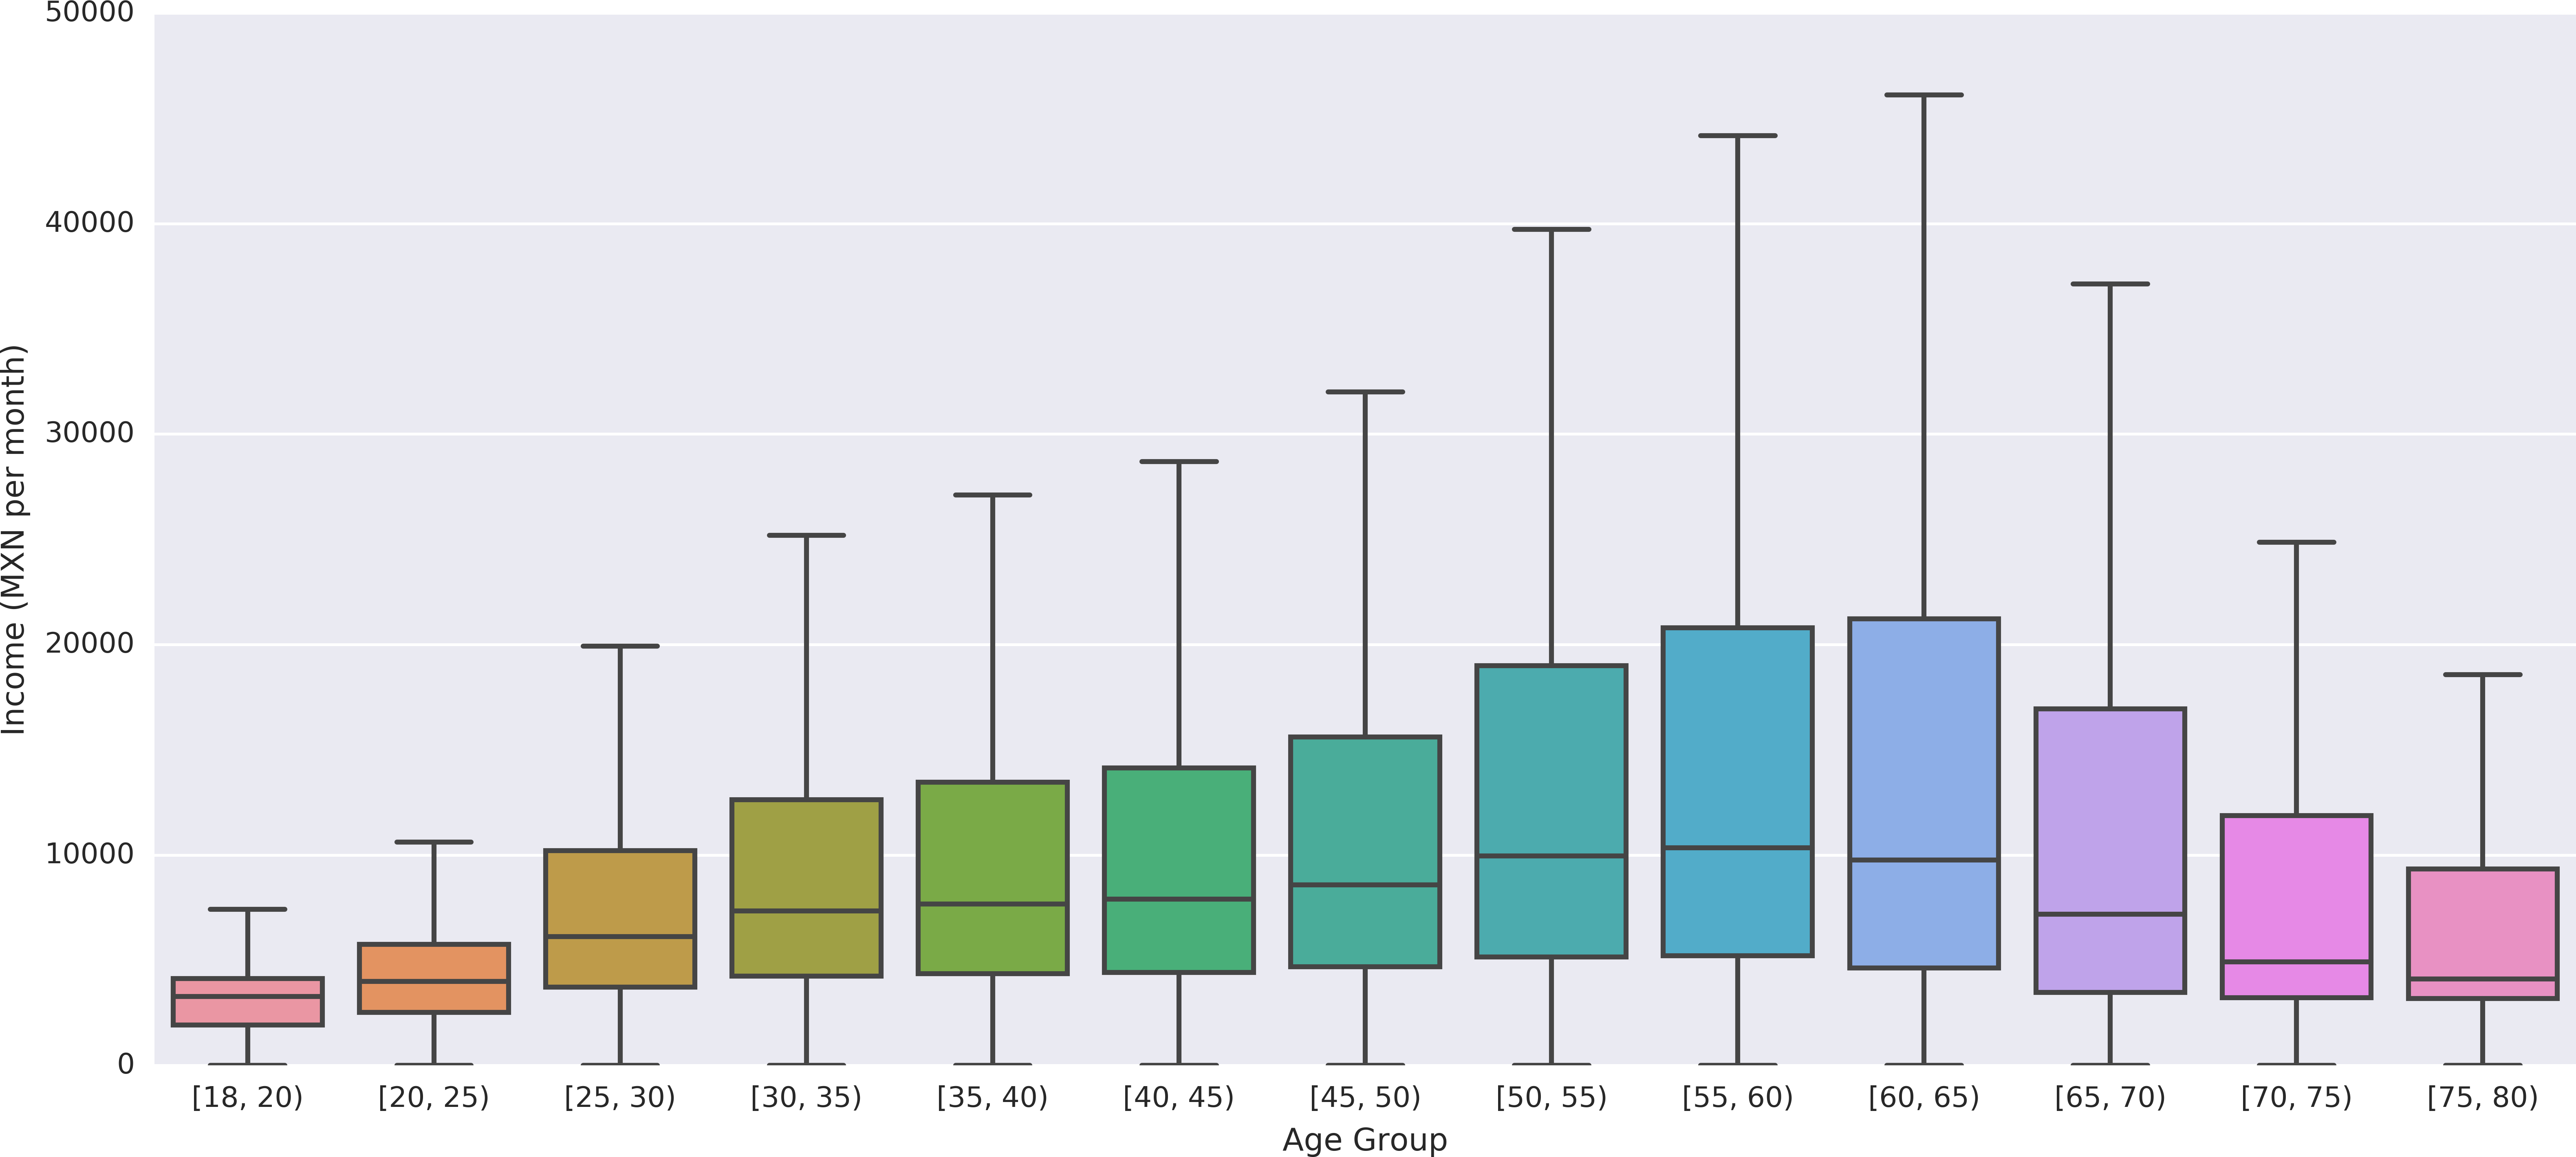
\includegraphics[width=\columnwidth]{figures/income_age_boxplot4/income_age_boxplot4_wide.png}
\caption{Distribution of income $b_s$ according to age $b_a$}
\label{income_age_boxplot}
\end{center}
\end{figure}
This is consistent with data from~\cite{gallup2013}.

\end{frame}




\begin{frame}{Uneven Income Distribution}

\begin{figure}
\begin{center}
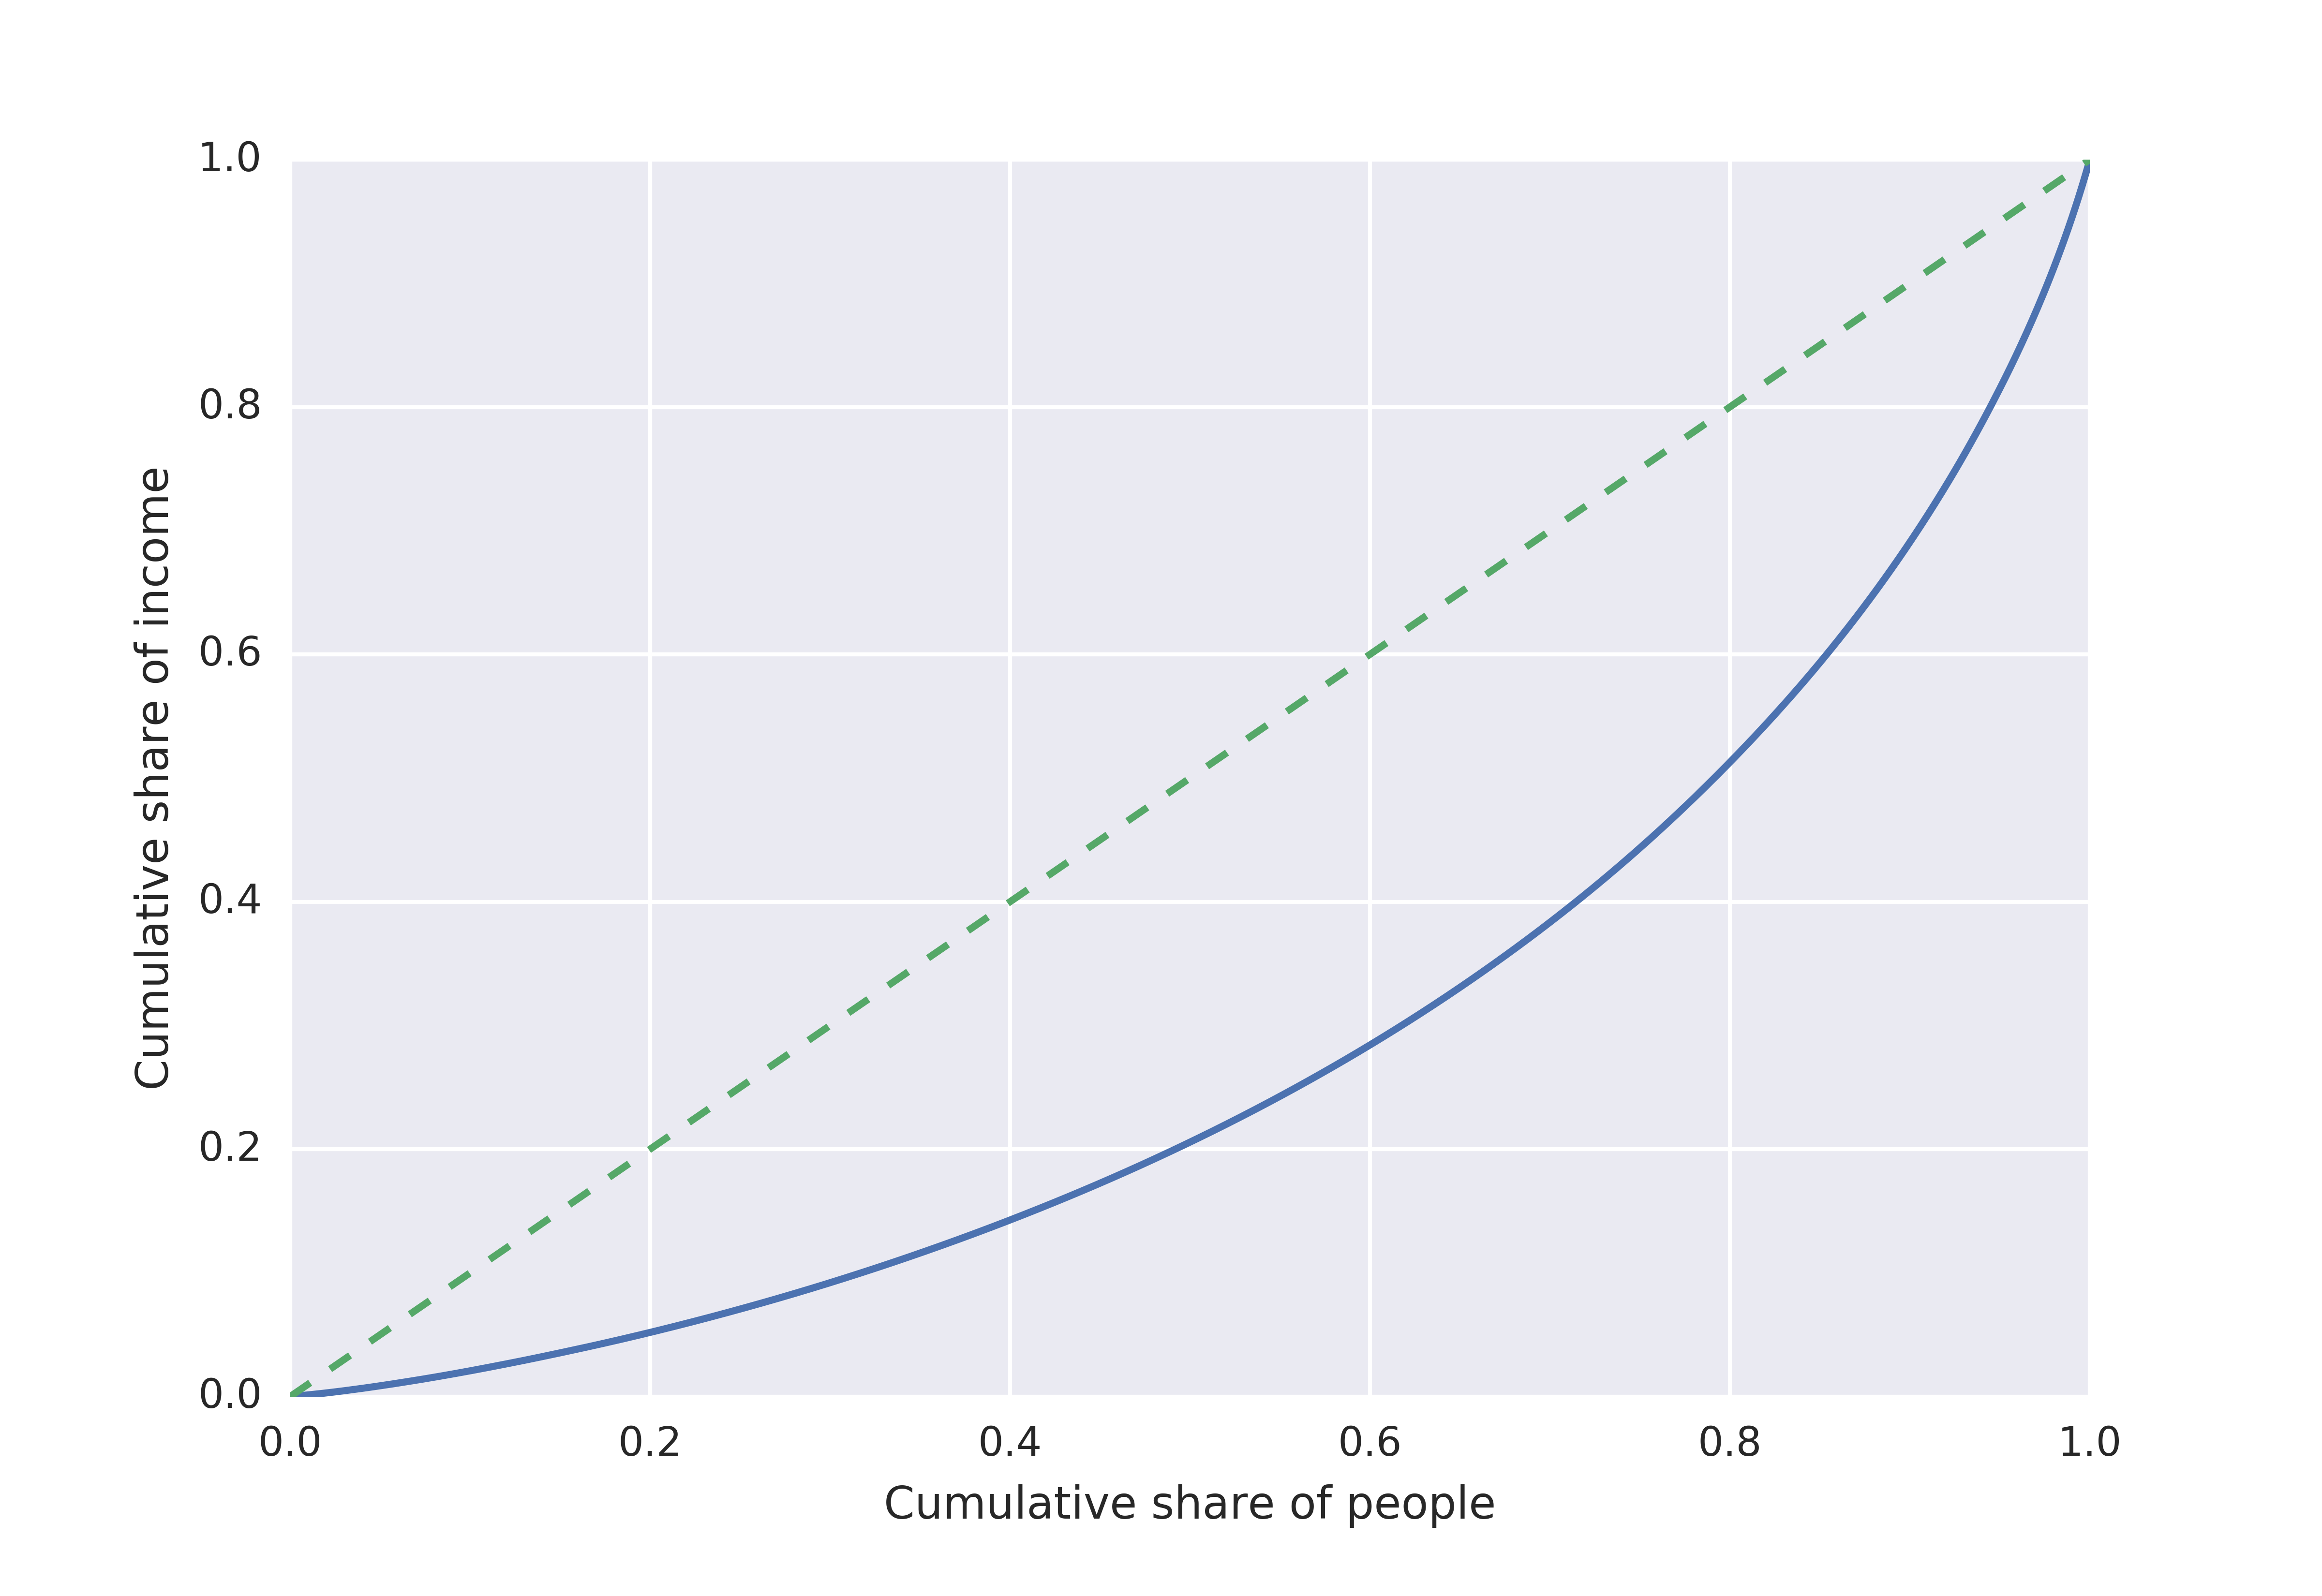
\includegraphics[width=0.8\columnwidth]{figures/cumulative_income.png}
\caption{Lorenz curve representing the distribution of income of bank clients}
\label{fig:income_distribution}
\end{center}
\end{figure}

\end{frame}


\begin{frame}{Gini Coefficient}

\begin{columns}
\begin{column}{0.45\textwidth}

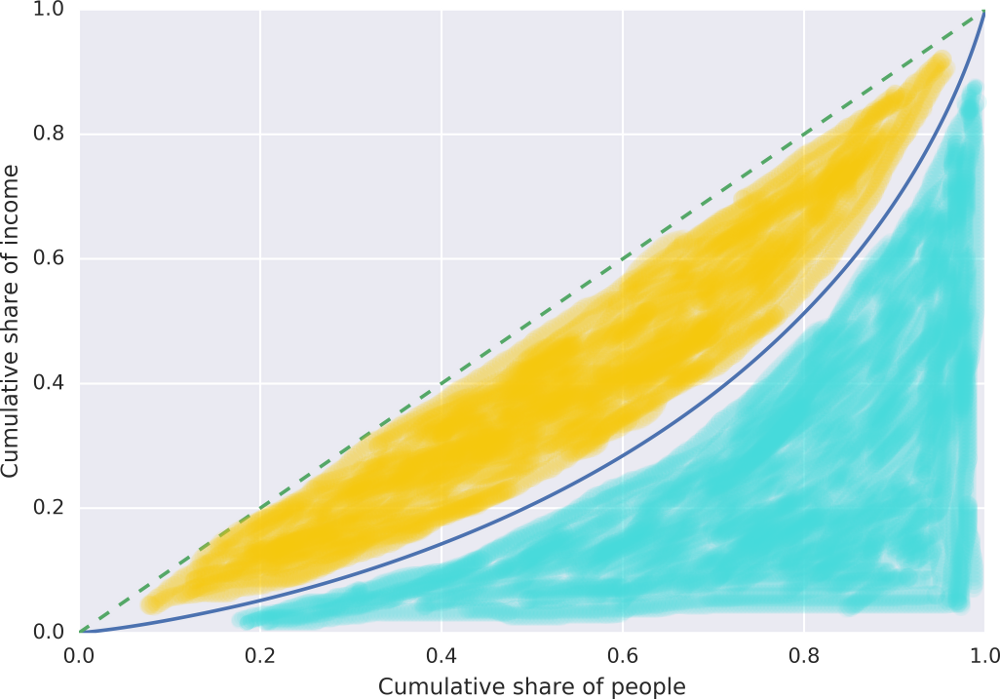
\includegraphics[width=\columnwidth]
{cumulative_income_gini.png}

\end{column}
\begin{column}{0.54\textwidth}

From the Lorenz curve, we can compute the Gini coefficient:
$$G = 0.45$$

According to the World Bank~\cite{world_bank}, the Gini coefficient for whole Mexico was \num{0.481} in 2012. 

\end{column}
\end{columns}
\medskip
\medskip

Top 10\% accumulate 33\%    of total income.\\
Top 20\% accumulate 50.5\%  of total income. \\
Top 30\% accumulate 63.1\%  of total income.

\end{frame}


%%%%%%%%%%%%%%%%%%%%%%%%%%%%%%%%%%%%%%%%%%%%%%%%%%%%%%%%%%%%%%%%%%%%%%%%%%%%%%%%%%%%%%%%%%%%%%%%%%%%%%%%%%%%
\section{Income Prediction}
%%%%%%%%%%%%%%%%%%%%%%%%%%%%%%%%%%%%%%%%%%%%%%%%%%%%%%%%%%%%%%%%%%%%%%%%%%%%%%%%%%%%%%%%%%%%%%%%%%%%%%%%%%%%

\begin{frame}{What do we use?}

\centering

\begin{LARGE}
Individual features~?

\bigskip

or

\bigskip
\medskip

Network topology~??
\end{LARGE}
\end{frame}


\begin{frame}{Income Homophily}

\begin{figure}[h]
\begin{center}
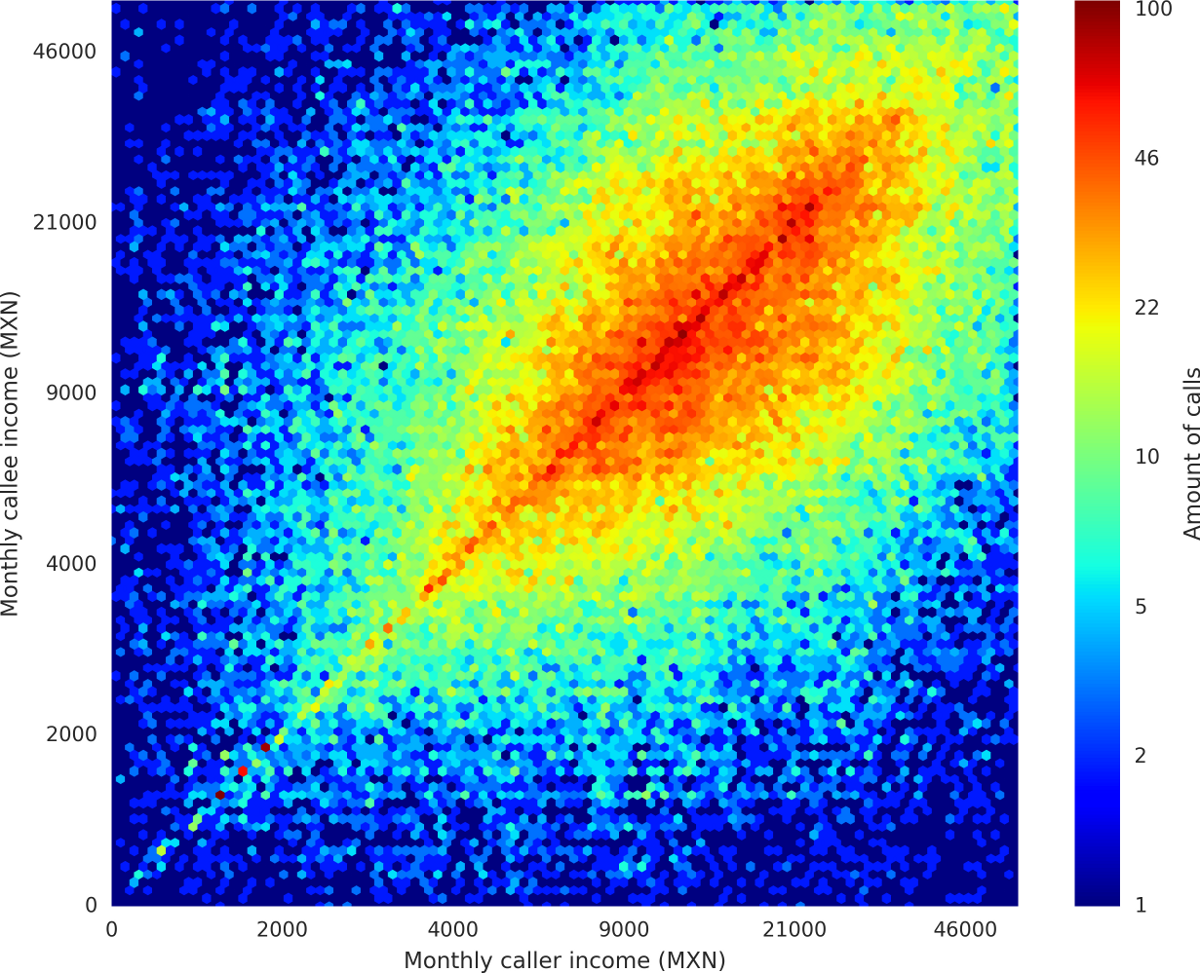
\includegraphics[width=0.7\columnwidth]{Homophily_income_origin_target_low.png}
\caption{Number of calls between users, according to their monthly income}
\label{homophily_heatmap}
\end{center}
\end{figure}

Similar to homophily with respect to age in~\cite{brea2014}.

\end{frame}

\begin{frame}{What do we predict?}

Instead of predicting the exact value of a user's income, our strategy is to distinguish between 2 categories:
\begin{itemize}
\item $R_1 = \closeopen{1000}{6300}$ i.e.\ low income
\item $R_2 = \closeopen{6300}{\infty}$ i.e.\ high income
\end{itemize} 

\bigskip

We place users into two distinct groups $ H_1, H_2 \subseteq G$:
\[
	g \in H_i \iff g_s \in R_i
\]

\end{frame}


\begin{frame}{Bayesian inference}

\begin{itemize}
\item Reason with \textbf{uncertainty}.
\bigskip
\item Philosophy: treat anything uncertain as random, described by a probability distribution.
\bigskip
\item Given observations, we want to infer the best parameters of the probability distribution.

\end{itemize}
\end{frame}

\begin{frame}{The Theorem of Bayes (and notation)}
$$
P(H | E) = \frac{P(E | H) \cdot P(H)}{P(E)}
$$
where
\begin{itemize}
\item $E$ is the new \textcolor{blue}{evidence} (observation).
\item $H$ is the \textcolor{blue}{hypothesis} to be tested with data (prior to evidence).
\item $P(H)$ is the \textcolor{blue}{prior} probability of H before E if observed.
\item $P(E | H)$ is the \textcolor{blue}{likelihood} of observing E.
\item $P(E)$ is the marginal likelihood (does not depend on H).
\item $P(H | E)$ is the \textcolor{blue}{posterior} probability (what we want to know!)
\end{itemize}
\end{frame}


\begin{frame}{How do we predict?}
\begin{block}

\begin{itemize}

\item $Q = $ users having at least one connection link to bank clients.

\item $\forall q^j \in Q$, we compute the number of outgoing calls $a^j_i$ to the category $H_i$.

\item Idea: A person is usually in the same income category as the majority of people it calls.
\end{itemize}
\end{block}
\pause

\begin{block}

\begin{itemize}
\item We use a continuous prior probability distribution called
the Beta distribution.

\item We use the amount of calls $a^j_i$  as parameters defining a Beta distribution for the probability of belonging to a given category.
\end{itemize}
\end{block}

\end{frame}



\begin{frame}{Motivation}

\begin{columns}
\begin{column}{0.49\textwidth}

\begin{figure}[h]
\begin{center}
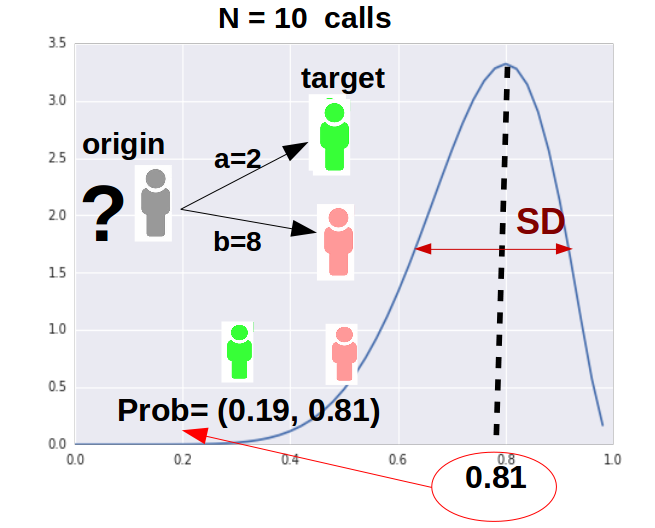
\includegraphics[width=\columnwidth]{distribucion1.png}
\end{center}
\end{figure}
\end{column}

\begin{column}{0.49\textwidth}

\begin{figure}[h]
\begin{center}
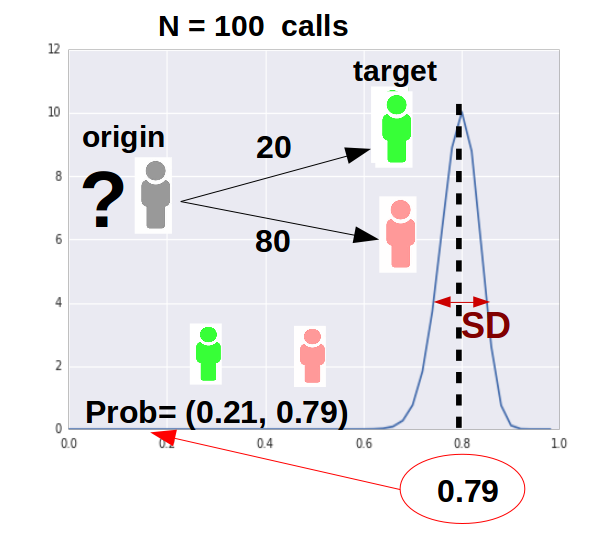
\includegraphics[width=\columnwidth]{distribucion2.png}
\end{center}
\end{figure}

\end{column}
\end{columns}

\medskip

The frequency of calls (to category 1 and 2) loses information.

We want to compare distributions.

\end{frame}



\begin{frame}{Beta Distribution}

We define \(\Beta^j\) as the Beta probability distribution function for each user:
\begin{equation}
	\Beta^j \left( x; \alpha^j, \beta^j \right) = \frac{1}{\Beta \left( \alpha^j, \beta^j \right)} x^{\alpha^j - 1} \cdot {\left( 1 - x \right)}^{\beta^j - 1}
\label{Beta}
\end{equation}
where $\alpha^j = a^j_1 +1$ and $\beta^j = a^j_2 +1$ are the parameters of the Beta distribution,
and $\Beta$ is the beta function, defined as:
\begin{equation}
\Beta \left( \alpha, \beta \right) =
\frac{\Gamma \! \left( \alpha \right) \cdot \Gamma \! \left( \beta \right)}
{\Gamma \! \left( \alpha + \beta \right)}
\label{Beta}
\end{equation}

We obtain a Beta distribution for the probability of belonging to high income category (for each user).

\end{frame}



\begin{frame}{Determining the category}

	\begin{columns}
		\begin{column}{0.49\textwidth}

\begin{figure}[h]
\begin{center}
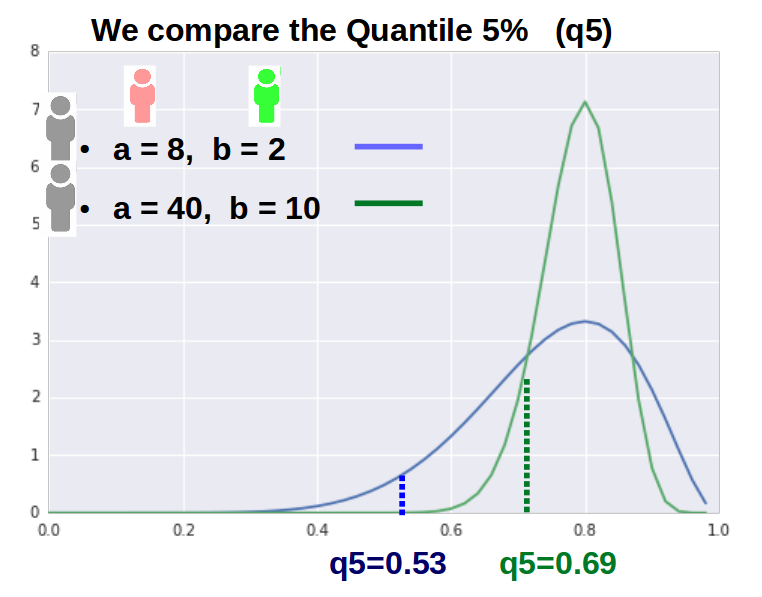
\includegraphics[width=\columnwidth]{distribucion3.png}
% \caption{Tres.}
\end{center}
\end{figure}
\end{column}

\begin{column}{0.49\textwidth}

\begin{figure}[h]
\begin{center}
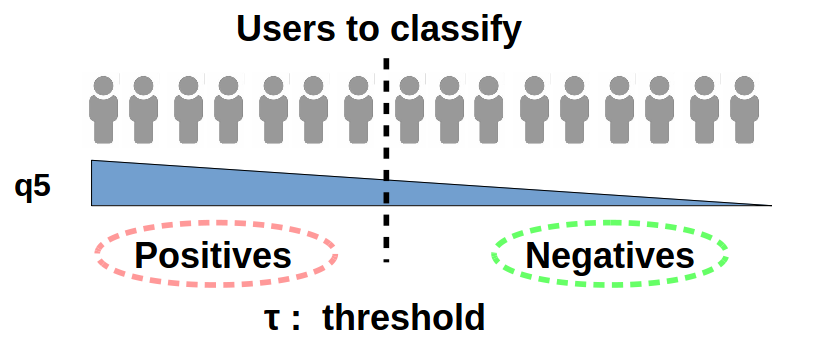
\includegraphics[width=\columnwidth]{distribucion4.png}
% \caption{Cuatro.}
\end{center}
\end{figure}

\end{column}
\end{columns}


\begin{itemize}

\item Find the lowest 5 percentile $q5$ for this probability. 

\item If $q5$ is above threshold $\tau$, we assign user to $H_2$.

\item Take into account both the mean and the broadness (uncertainty) of the distribution. 

\item Category assigned to a user depends on its Beta distribution and on our choice of $\tau$.
\end{itemize}

\end{frame}

%%%%%%%%%%%%%%%%%%%%%%%%%%%%%%%%%%%%%%%%%%%%%%%%%%%%%%%%%%%%%%%%%%%%%%%%%%%%%%%%%%%%%%%%%%%%%%%%%%%%%%%%%%%%
\section{Results}
%%%%%%%%%%%%%%%%%%%%%%%%%%%%%%%%%%%%%%%%%%%%%%%%%%%%%%%%%%%%%%%%%%%%%%%%%%%%%%%%%%%%%%%%%%%%%%%%%%%%%%%%%%%%

\begin{frame}{Evaluation of Performance}

We examine:
\begin{itemize}
\item true positive rate \( \TPR = \TP / \operatorname{P} \)
\item false positive rate \( \FPR = \FP / \operatorname{N} \)
\end{itemize}
Where:
\begin{itemize}
\item $\TP$ is the number of correctly predicted users with high income,
\item $\operatorname{P}$ is the total number of users with high income, 
\item $\FP$ is the number of users incorrectly classified as having high income,
\item $\operatorname{N}$ is the total number of users with low income.

\end{itemize} 


\end{frame}

\begin{frame}{ROC Curve}

\begin{figure}
\begin{center}
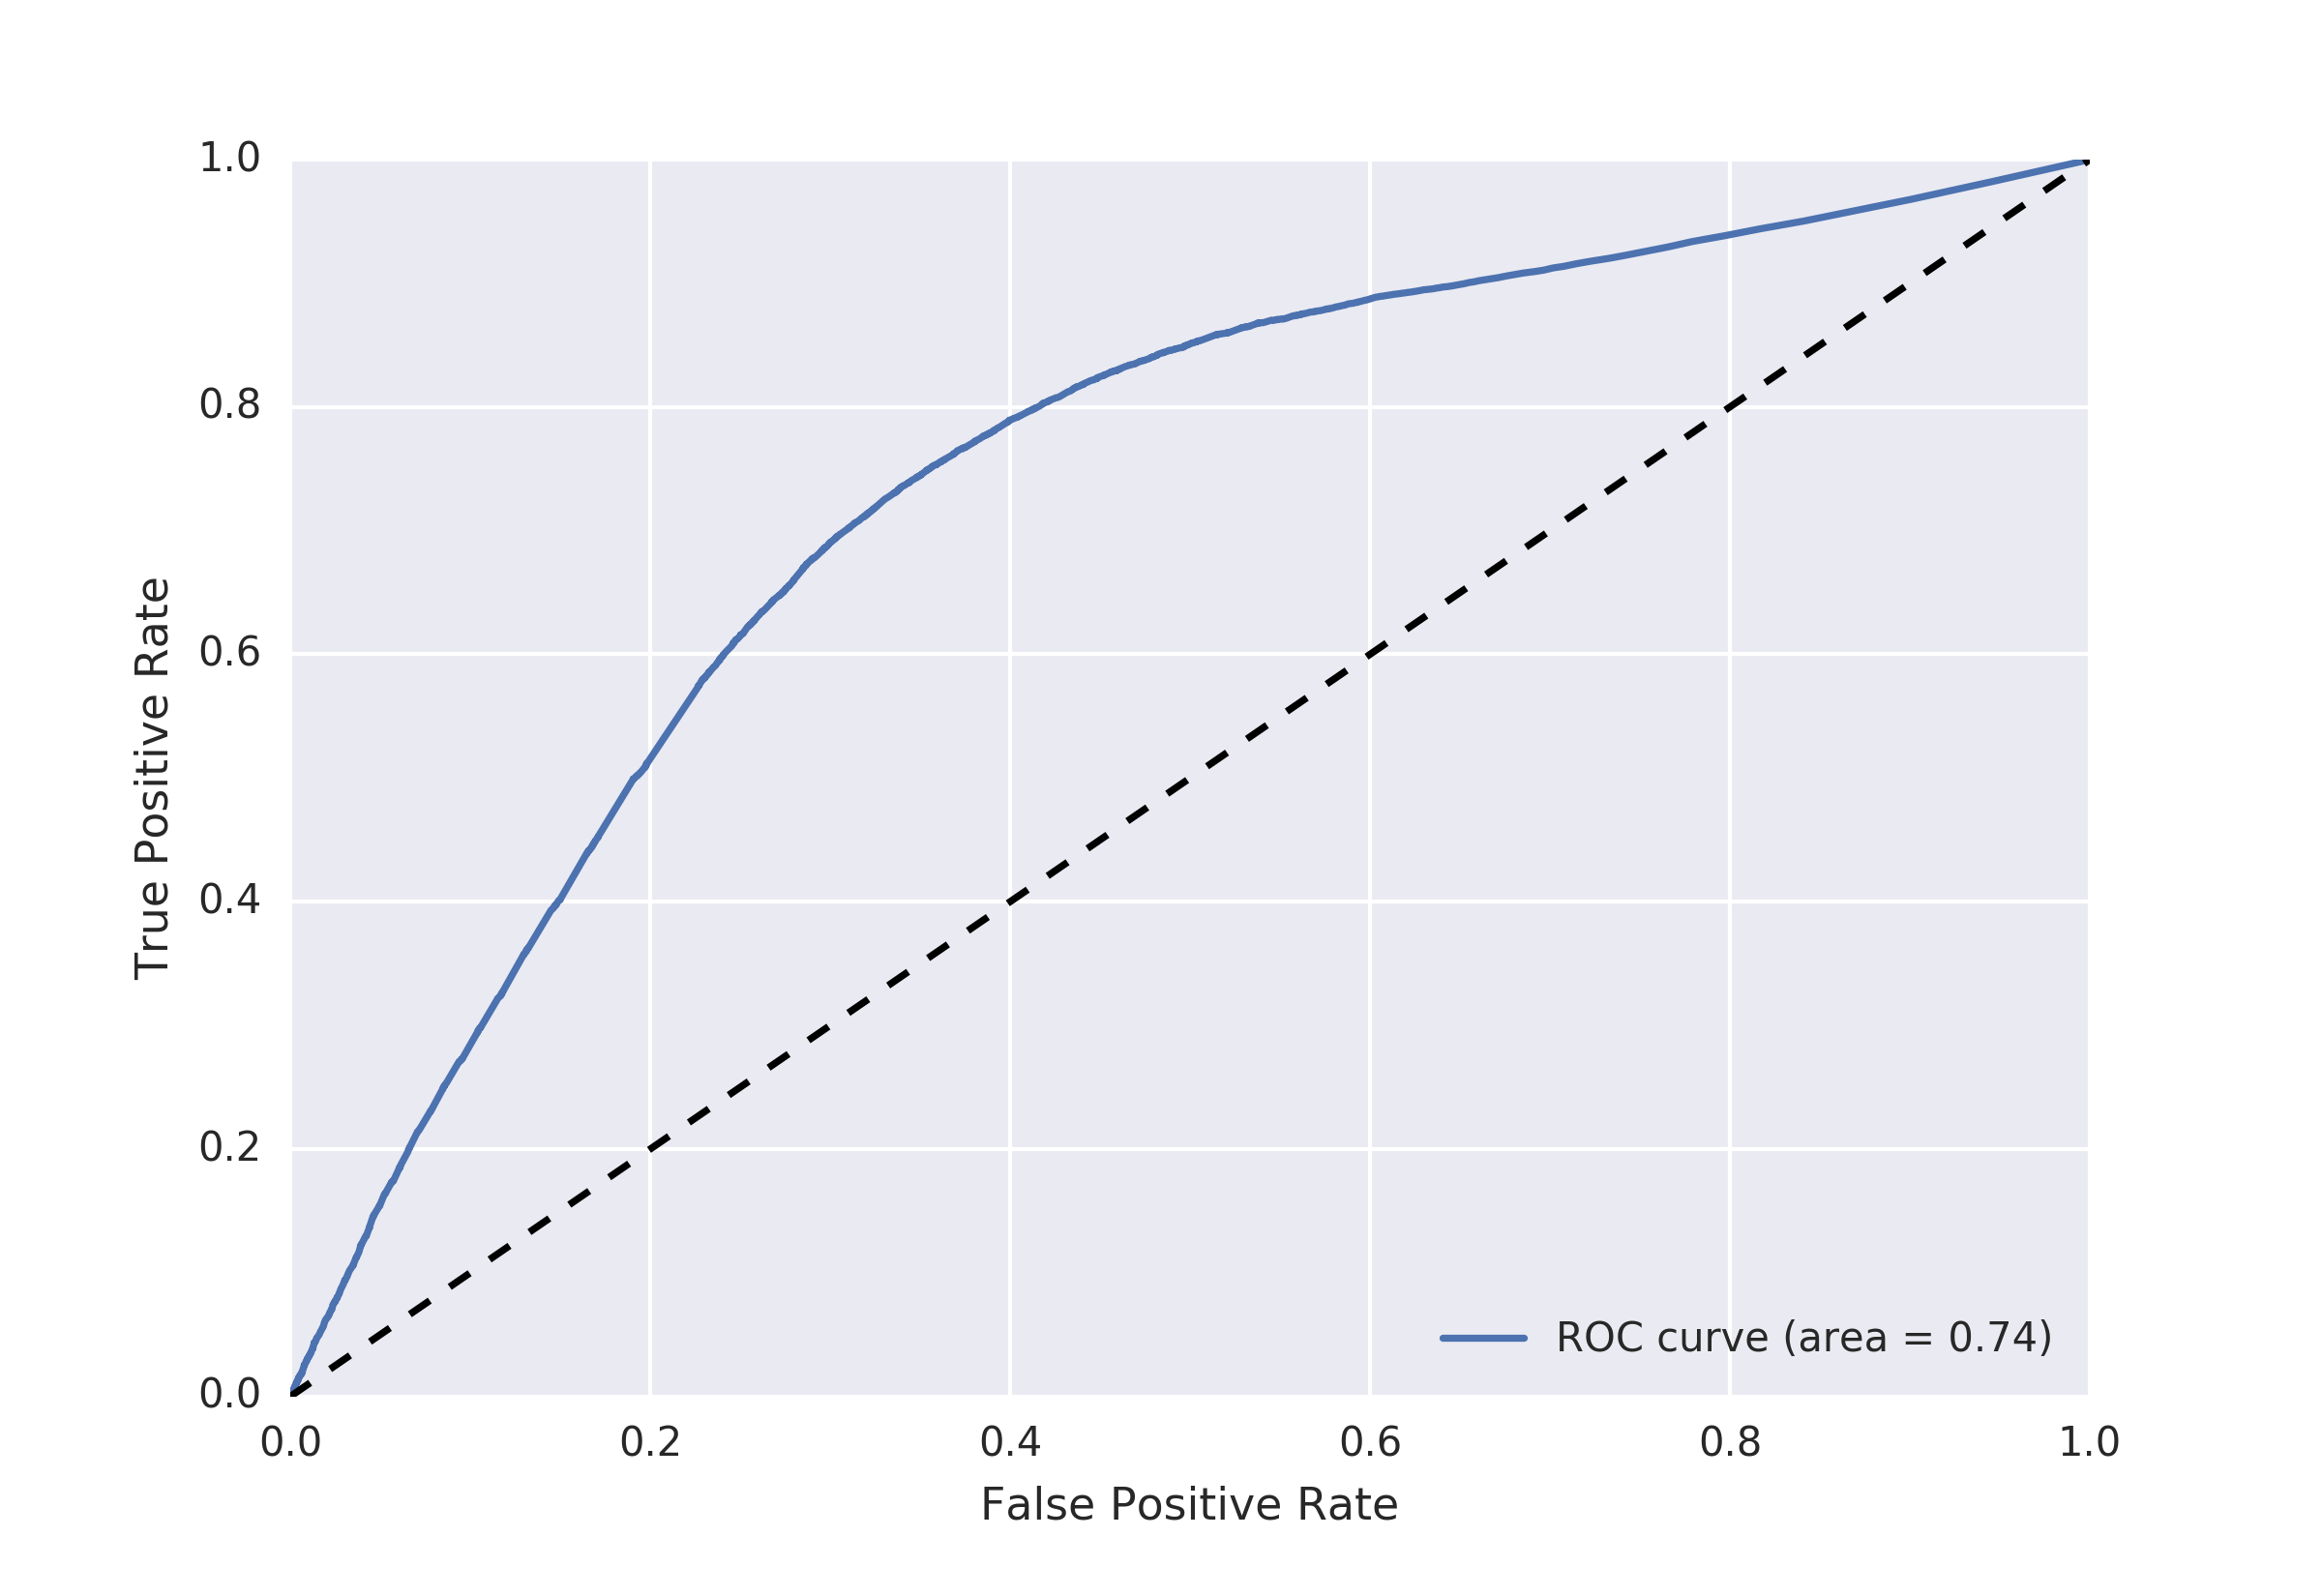
\includegraphics[width=0.7\columnwidth]{figures/ROC_BETA/ROC_Beta_based_approach_201504.png}
\caption{ROC curve for prediction procedure}
\label{ROC_multiclass}
\end{center}
\end{figure}

We observed an $\AUC = 0.74$ indicating that our predictor is better than a random predictor ($\AUC \simeq 0.50$).

\end{frame}


\begin{frame}{Accuracy}

\begin{figure}[p]
\begin{center}
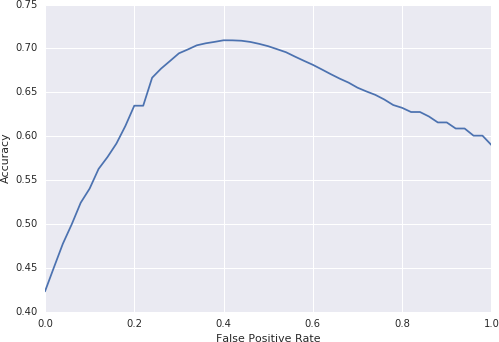
\includegraphics[width=0.7\columnwidth]{figures/accuracy_vs_fpr.png}
\caption{Accuracy as a function of FPR}
\label{fig:accuracy_vs_fpr}
\end{center}
\end{figure}

The best accuracy obtained is \num{0.71} for $\tau = 0.4$.

\end{frame}

\begin{frame}{Comparison with Other Methods}

We applied two other inference methods to the same data and compared their accuracies to our Bayesian model.

\begin{itemize}
	\item \textbf{Random selection} which chooses randomly the category for each user.
	The accuracy is as expected \num{0.5}.
	\item \textbf{Majority voting} which decides the category depending on the category of the majority of its contacts.
	The accuracy for majority voting is \num{0.66}.
	\item \textbf{Bayesian method} gives an accuracy of \num{0.71}.
\end{itemize}

\end{frame}


\begin{frame}{Extension to Multiple Categories}

\begin{figure}[h]
\begin{center}
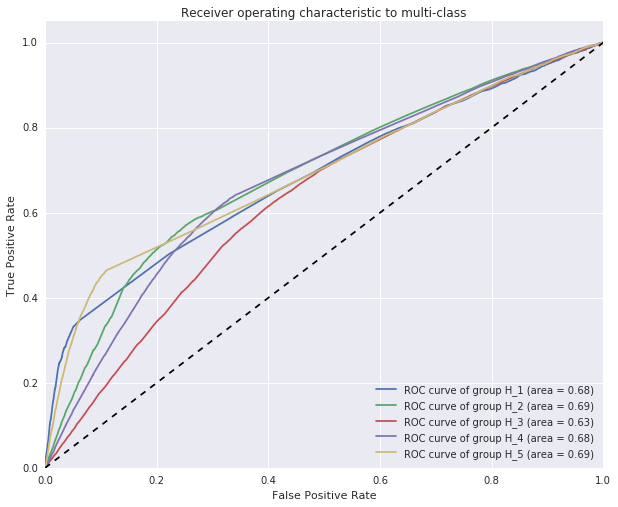
\includegraphics[width=0.6\columnwidth]{figures/ROC_multiclass/ROC_multiclass.png}
\caption{ROC curves for multiclass problem}
\end{center}
\label{roc_multiple_categories}
\end{figure}

We use the Dirichlet distribution for the probability of belonging to multiple categories.
% The performances observed are: $\AUC_1 = 0.68$, $\AUC_2 = 0.69$, $\AUC_3 = 0.63$, $\AUC_4 = 0.68$, $\AUC_5 = 0.69$.

\end{frame}

\begin{frame}{References}
\justifying%
\scalefont{0.6}
\bibliographystyle{unsrtnat}
\bibliography{../bibliography/sna}
\end{frame}

\begin{frame}{That's all folks!}
\centering
\begin{huge}
Thank you!
\end{huge}

\bigskip
\bigskip
\begin{Large}

Carlos Sarraute

\bigskip

\texttt{charles@grandata.com}
\end{Large}

\end{frame}

\end{document}

